\newpage
\section{Лекция 18}
\subsection{Задача линейного программирования}
Пусть \[\bar x=\begin{pmatrix}
x_1\\
\vdots\\
x_n\\
\end{pmatrix} \in \mathbb{R}^n\]
Нужно максимизировать линейную функцию $$f(\bar x)=c_1x_1+\cdots +c_nx_n \to max $$ при ограничениях
\begin{center}
    $
    \left\{
    \begin{array}{lcl}
    a_{11}x_1+\cdots +a_{1n}x_n \leqslant d_1\\
    \cdots\\
    a_{m1}x_1+\cdots +a_{mn}x_n \leqslant d_m\\
    \end{array}
    \right.
    $
\end{center}
$$A\bar x \leqslant \bar d$$
$$x_i \geqslant 0 \Leftrightarrow -x_i \leqslant 0$$
\begin{center}
    $x_1+x_2 \leqslant d$ и $x_1+x_2 \geqslant d~\Leftrightarrow~-x_1-x_2\leqslant -d~\Leftrightarrow~x_1+x_2=d$
\end{center}
\begin{center}
    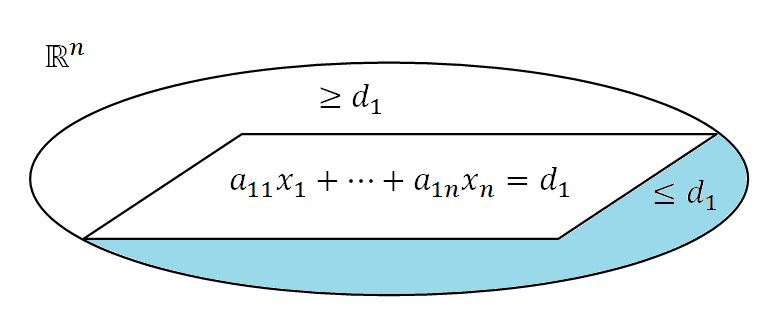
\includegraphics[scale=0.6]{l18_1.png}\\
\end{center}
Вариант:
\begin{center}
    $f(\bar x)=<\bar c, \bar x> \to min$\\
    $
    \left\{
    \begin{array}{lcl}
    A\bar x \leqslant \bar d \in \mathbb{R}^m\\
    \bar x \geqslant \bar 0 ~~(x_1\geqslant 0, \cdots, x_n \geqslant 0)\\
    \end{array}
    \right.
    $
\end{center}
\textbf{Задача о диете.}\\
Дано несколько продуктов $E_1, \cdots, E_n$ (еда) и информация о них, например, У -- углеводы, Б -- белки, К -- калории. Также дана цена каждого продукта (\$).\begin{center}
    \begin{tabular}{|c|c|c|c|c|}
        \hline
        & У & Б & К & Цена $\$$ \\ \hline
        $E_1$ &  & $\bar a_1$ &  & \\ \hline
        $\vdots$ &  & $\cdots$ &  & \\ \hline
        $E_n$ &  & $\bar a_n$ &  & \\ \hline
    \end{tabular}
\end{center}
Пусть $\bar y=(y_1, \cdots, y_n)$ -- количество употребленных единиц пищи каждого типа.\\
Ограничения:
$$<\bar a_i, \bar y> \geqslant c_i,~~i=1, \cdots, m$$
или 
\begin{center}
    $
    \left\{
    \begin{array}{lcl}
    A\bar y \geqslant \bar c\\
    \bar y \geqslant \bar 0\\
    \end{array}
    \right.
    $
\end{center}
Вектор цен: $\bar p=(p_1, \cdots, p_n)$ -- цены на $y_1, \cdots, y_n$.\\
Матрица $A$ имеет размер $m \times n$ 
\[A=\begin{pmatrix}
\bar a_1\\
\vdots\\
\bar a_m\\
\end{pmatrix}\]
Функция $f(\bar y)=<\bar p, \bar y>$.\\
Общая постановка:
\begin{center}
    $
    \left\{
    \begin{array}{lcl}
    A\bar y \geqslant \bar c\\
    \bar y \geqslant \bar 0\\
    f(\bar y)=<\bar p, \bar y> \to min\\
    \end{array}
    \right.
    $
\end{center}
Всего $\approx C_m^n$ вершин, то есть меньше $\cfrac{m^{m-n}}{n!}$.\\
\\
\textbf{Пример 1.}
\begin{center}
    \begin{tabular}{|c|c|c|c|c|}
        \hline
        & Б & Ж & У & Цена \\ \hline
        Мясо & 60 & 30 & 10 & 100\\ \hline
        Торт & 10 & 40 & 50 & 150\\ \hline
        Норма $c_i$ & 30 & 30 & 40 & \\ \hline
    \end{tabular}\\ ~\\
    $\bar a_1=(60, 10)$ -- белки\\
    $\bar a_2=(30, 40)$ -- жиры\\
    $\bar a_3=(10, 50)$ -- углеводы
\end{center}
$$A\bar y \geqslant \bar c$$
\[\begin{pmatrix}
60 & 10\\
30 & 40\\
10 & 50\\
\end{pmatrix}\begin{pmatrix}
y_1\\
y_2\\
\end{pmatrix} \geqslant \begin{pmatrix}
30\\
30\\
40\\
\end{pmatrix}\]
$$f(\bar y)=<\bar p, \bar y>=\bar p^T\bar y=100y_1+150y_2 \to min$$
$$60y_1+10y_2 \geqslant 30~~(1)$$
$$30y_1+40y_2 \geqslant 30~~(2)$$
$$10y_1+50y_2 \geqslant 40~~(3)$$
\begin{center}
    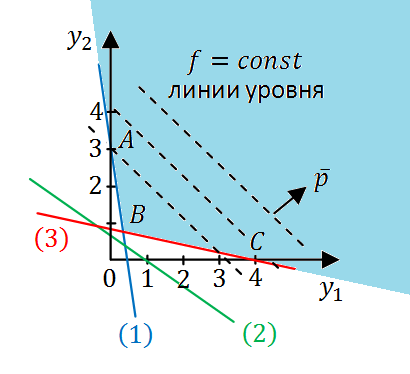
\includegraphics[scale=0.8]{l18_2.png}\\
\end{center}
Надо найти в какой вершине будет достигаться минимум функции $f(\bar y)$. Посмотрим значения в точках $A$, $B$ и $C$.\\
$$f(A)=100\cdot 0+3\cdot 150=450$$
$$f(C)=100\cdot 4+150 \cdot 0=400$$
$$f(B)=100y_1+150y_2$$
Наидем пересечение (1) и (3):
\begin{center}
    $
    \left\{
    \begin{array}{lcl}
    60y_1+10y_2=30\\
    10y_1+50y_2=40\\
    \end{array}
    \right.
    $
\end{center}
\begin{center}
    $
    \left\{
    \begin{array}{lcl}
    6y_1+y_2=3\\
    6y_1+30y_2=24\\
    \end{array}
    \right.
    $
\end{center}
$$y_2=\cfrac{21}{29},~~y_1=4-\cfrac{5\cdot 21}{29}=\cfrac{11}{29}$$
Получим
$$f(B)=100\cdot \cfrac{11}{29}+150\cdot \cfrac{21}{29}=\cfrac{4250}{29}\approx 147$$
Таким образом, наименьшее значение $f(\bar y)$ достигается в точке $B$ и принимает значение 147.
\subsection{Линейная производственная модель}
Пусть $\bar x$ -- выпуск $m$ видов продукции
\[\bar x=\begin{pmatrix}
x_1\\
\vdots\\
x_m\\
\end{pmatrix},\]
цены на эти виды продукции $$\bar c =(c_1, \cdots, c_m),$$
а доход $$\bar y=c_1x_1+\cdots +c_mx_m=<\bar c, \bar x> \to max$$
Имеются ресурсы $1, \cdots, n$ и указаны ограничения на них (запасы)
\[\bar d=\begin{pmatrix}
d_1\\
\vdots\\
d_n\\
\end{pmatrix}\]
$a_{ij}$ -- число единиц $j$ ресурса для производства единицы $i$ типа продукции. Для производства $x_i$ надо $x_ia_{i1}$ ресурса 1, $\cdots$, $x_ia_{ij}$ ресурса $j$, $\cdots$, $x_ia_{in}$ ресурса $n$.\\
Всего потратим ресурса $j$: $$x_1a_{1j}+\cdots+x_na_{nj}=\bar x^T A^j \leqslant d_j$$
ограничения: $$\bar x^TA\leqslant\bar d^T$$
Прямая задача:
\begin{center}
    $
    \left\{
    \begin{array}{lcl}
    \bar x^TA\leqslant \bar d ~~\Leftrightarrow ~~A^T\bar x\leqslant \bar d\\
    \bar x \geqslant 0\\
    g(\bar x)=<\bar c, \bar x>=c_1x_1+\cdots+c_mx_m \to max\\
    \end{array}
    \right.
    $
\end{center}
Пусть $\bar x^*\in \mathbb{R}^m$ -- оптимальное решение, такое что $g_{max}=<\bar c, x^*>$.\\
\begin{center}
    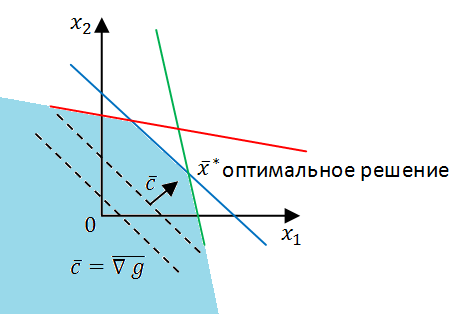
\includegraphics[scale=0.84]{l18_3.png}\\
\end{center}
Двойственная задача линейного программирования.\\
Дано:
\begin{center}
    $
    \left\{
    \begin{array}{lcl}
    A\bar y\geqslant 0, \bar c\in \mathbb{R}^m, \bar y \in \mathbb{R}^n, A_{m\times n}\\
    \bar y \geqslant 0\\
    f(\bar y)=<\bar d, \bar y> \to min\\
    \end{array}
    \right.
    $
\end{center}
Тогда $y^*$ -- решение, то есть $f(y^*)=<d, \bar y^*>=f_{min}$.
\begin{theorem}[Основная двойственности]
    \ 
\begin{enumerate}
    \item Если $\bar x$ -- допустимый для прямой задачи, а $\bar y$ -- допустимый для двойственной задачи, то $$g(x)\leqslant f(y), ~<c, x>\leqslant <d, y>$$
    \item Если $x^*, y^*$ -- решения прямой и двойственной задач, то $f(y)=g(x)$, то есть $$<c, x^*>=<d, y^*>=f_{min}=g_{max}$$
\end{enumerate}
\end{theorem}
\begin{proof}\ 
    \begin{enumerate}
        \item \ 
        \begin{center}    
        $
        \left\{
        \begin{array}{lcl}
        x^TA \leqslant d^T\\
        Ay\geqslant c\\
        \end{array}
        \right.
        $
        \end{center}
        $$<c, x>=x^Tc\leqslant x^TAy \leqslant d^Ty=f(y)=<d, y>$$
        \item 
        Так как значения оптимальны, то вместо неравенств в доказательстве пункта 1 теоремы везде будут стоять равенства, потому что $<x^TA, y^*>=<d^T, y^*>$, либо они несущественны и равны 0. Значит $<c, x^*>=<d, y^*>$
    \end{enumerate}
\end{proof}